\subsection{Model-complexity and model-selection}

\subsubsection{SMV v.s. Perceptron}

In this section we try to compare the performances of the Perceptron, we implemened during the first assignment against the SVM from this one.
Since the Perceptron can only handle linearly separable data, we will use a SVM with hard margin and linear Kernel for this comparison.
\\
\\
To select a proper test set we selected $M = 150$ training sets $\tau _{k},k \in \{1,\ldots,M\}$ form the MNIST training set with no more than $N = 70$ images each.
For $k \in \{1,\ldots,M\}$ we trained both SVM and Perceptron using $\tau_k$ and calculated the test error rate $R_k$ on the {MNIST} test set - again for both SVM and Perceptron.
\\
\\
The average error $R_{avg} = \frac{1}{M}\sum_{k=1}^M R_k$ of SVM and Perceptron can be seen in the table below (\ref{tab:avg_error}).
Figure \ref{fig:error_SVM_perc} shows $\tau_k$.

\begin{table}[!h]
\begin{tabular}{lll}
 \textbf{$R_{avg}$ SVM} & \textbf{ $R_{avg}$ Perceptron} \\
 0.07329339987931965       &     0.028047619047619037      \\
\end{tabular}
\caption{\label{tab:avg_error} $R_{avg}$ for both algorithms }
\end{table}

\begin{figure}[!h]
\begin{center}
\centering
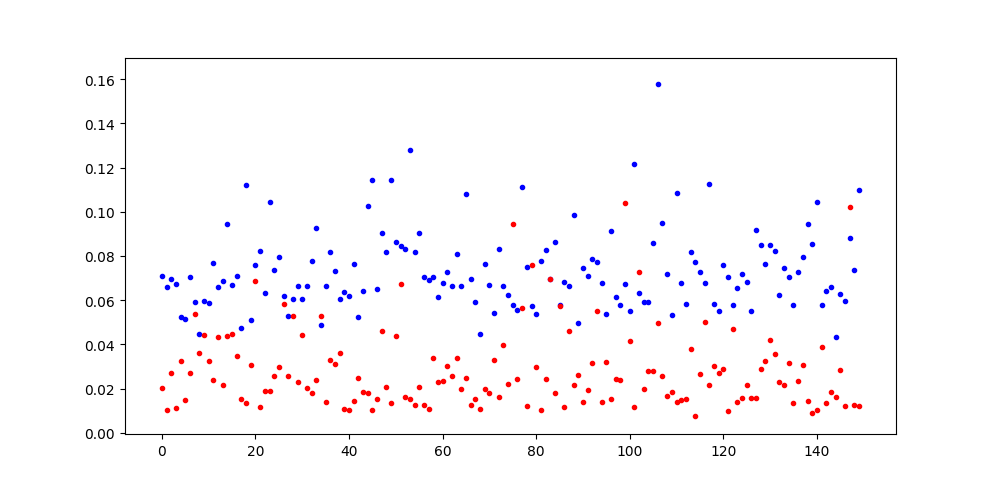
\includegraphics[width=1\textwidth]{figures/lin_svm_perc_error.png}
\end{center}
\caption{\label{fig:error_SVM_perc} Comparing the error rates of $\tau_k$ from SVM (blue) against Perceptron(red) }
\end{figure}

Against our expectations SVM does not perform as well as suspected, which could be due to the use of the linear Kernel and $C=\infty$ (no slack variables).

\subsubsection{Tuning meta-parameters}